\section{Teorio}

\subsection{Sciigoj}

%%%>>>>>>>>>>>>>>>>>>>>>>>>>>>>>>>>>>>>>>>>>>>>>>>>>>>>>>>>>>>>>>>>>>>>>>>>>>>>>>>>>>>>>>>>>>>>>>
  \begin{frame}
    \frametitle{Informado/spamado ekvilibro?}
	\framesubtitle{Ĝenerale...}	
	\pause
	\begin{block}{I}
		Kiam iu afero rilatas al vi, vi volas esti informata.
	\end{block}
	\pause
	\begin{block}{II}
		Kiam afero ne rilatas al vi, vi ne volas aŭdi pri ĝi.
	\end{block}
	\pause
	\begin{block}{III}
		Tamen en libera tempo estus bone havi eblecon trarigardi, kio okazas.
	\end{block}
	
  \end{frame}
%%%<<<<<<<<<<<<<<<<<<<<<<<<<<<<<<<<<<<<<<<<<<<<<<<<<<<<<<<<<<<<<<<<<<<<<<<<<<<<<<<<<<<<<<<<<<<<<<


%%%>>>>>>>>>>>>>>>>>>>>>>>>>>>>>>>>>>>>>>>>>>>>>>>>>>>>>>>>>>>>>>>>>>>>>>>>>>>>>>>>>>>>>>>>>>>>>>
  \begin{frame}
    \frametitle{Kio estas sciigo en Trello?}

	\begin{enumerate}
		\item Sendita retposhtmesaĝo (\alert{agordeblas kiom ofte})
		\item Novaĵoj ĉe trello.com
		\item Android/iPhone
		\item "desktop" (??)
	\end{enumerate}
  \end{frame}
%%%<<<<<<<<<<<<<<<<<<<<<<<<<<<<<<<<<<<<<<<<<<<<<<<<<<<<<<<<<<<<<<<<<<<<<<<<<<<<<<<<<<<<<<<<<<<<<<



%%%>>>>>>>>>>>>>>>>>>>>>>>>>>>>>>>>>>>>>>>>>>>>>>>>>>>>>>>>>>>>>>>>>>>>>>>>>>>>>>>>>>>>>>>>>>>>>>
  \begin{frame}
    \frametitle{Agordoj de sciigoj}
	\begin{columns}
    \column{0.5\textwidth}
	    \begin{block}{Unue eniru agordojn}
	    	\begin{center}
	     	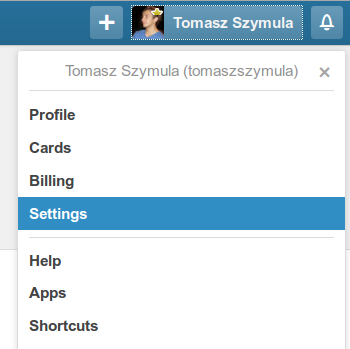
\includegraphics[scale=0.35]{ekranoj/eniru-agordojn}
	    	\end{center}
    	\end{block}
	\column{0.5\textwidth}
    	\begin{block}{Kaj trovu ĝustan sekcion}
    		\begin{center}
    		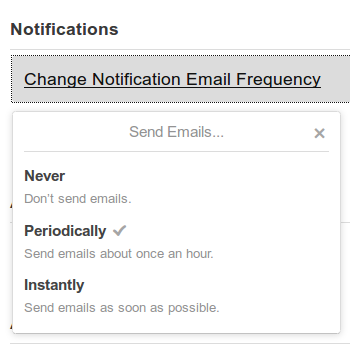
\includegraphics[scale=0.35]{ekranoj/sciigoj-agordo}
    		\end{center}
    	\end{block}

	\end{columns}
  \end{frame}
%%%<<<<<<<<<<<<<<<<<<<<<<<<<<<<<<<<<<<<<<<<<<<<<<<<<<<<<<<<<<<<<<<<<<<<<<<<<<<<<<<<<<<<<<<<<<<<<<